\documentclass[conference]{IEEEtran}
\usepackage[T1]{fontenc}
\usepackage{graphicx}
\usepackage{amsmath}
\usepackage{booktabs}
\usepackage{array}
\usepackage{url}
\usepackage{cite}
\usepackage{etoolbox}
% keep every table inside the two-column text width
\AtBeginEnvironment{table}{\footnotesize\setlength{\tabcolsep}{3pt}}

\begin{document}

\title{Recall-Constrained Alert Triage Across SOCs:\\
Statistical Threshold Calibration}

\author{\IEEEauthorblockN{Visweshwaran K}
\IEEEauthorblockA{\textit{School of Electronics Engineering} \\
\textit{Vellore Institute of Technology}\\
Chennai, India \\
visweshwaran.k2024@vitstudent.ac.in}
\and
\IEEEauthorblockN{Dr.\ Rishikeshan C A}
\IEEEauthorblockA{\textit{School of Computer Science and Engineering} \\
\textit{Vellore Institute of Technology}\\
Chennai, India \\
rishikeshan.ca@vit.ac.in}}

\maketitle

\begin{abstract}
Security operations centers (SOCs) receive far more alerts than analysts can review, and triage tools
are usually judged by a single score, F1, on one dataset. We examine whether that is sufficient,
using alerts from a Wazuh deployment that we attacked ourselves (969 labelled alerts) and the public
AIT Alert Data Set (eight simulated enterprise scenarios). Three findings emerge. First, a high F1
can be obtained by flagging nearly every alert, which saves analysts no work; at realistic attack
rates such systems are close to flagging everything. Second, results do not carry over between
environments: the ranking of an LLM, a rule-level threshold and trained classifiers differed between
the datasets, and thresholds chosen in one environment often missed the recall target in another.
Third, a classical order-statistic tolerance bound can select a threshold from a small random sample
of analyst-labelled alerts, with at least 90\% recall at 90\% confidence under stated assumptions. In
simulations on public alert streams totalling about 390,000 alerts, it reached an average coverage
of 96.5\% in the settings where it could certify, at the cost of clearing fewer benign alerts than a
naive threshold. A live implementation shows that the calibration workflow is feasible and that the
threshold is sensitive to labelling errors. The results support evaluating at realistic attack
rates, recalibrating for each environment, and checking labels before relying on a recall
guarantee.
\end{abstract}

\begin{IEEEkeywords}
alert triage, security operations center, SIEM, alert fatigue, threshold calibration, recall guarantee, LLMs
\end{IEEEkeywords}

\section{Introduction}

When detection rules are triggered, SIEM systems raise alerts. The volume of alerts is too high
for the number of analysts, and most alerts are false positives, which leads to alert fatigue and
missed attacks~\cite{alahmadi2022}. Mitigations either adjust the SIEM's own risk scoring and thresholds or use
machine learning~\cite{feng2017,ban2023,kapera2025,uetz2026} and, more recently, LLMs~\cite{xu2024llmsec} for the triage
decision. These methods are typically
tested with F1 or accuracy on one dataset~\cite{arp2022} and then deployed in an environment with a different
attack rate, hosts and logs. We ask: (i) does a high F1 on a test set with many attacks actually
mean that the analysts' workload is reduced? (ii) Does the ranking of the methods (rule-level
threshold, trained classifiers, an LLM) hold across datasets? (iii) When a model moves to a new
environment, how should its threshold be set, and what can be said about the attacks it catches? We also test whether LLMs, which are costly to run, beat cheap baselines.

\textbf{Contributions.} (1) An analysis, with projection to realistic attack rates, showing that
a high F1 can come from flagging everything. (2) A replication on the public AIT data~\cite{ait2023,landauer2024}, where an LLM
is on par with trained models and far above the rule-level threshold, unlike on our data. (3)
Evidence on both datasets that thresholds do not transfer. (4) An evaluation of a classical
distribution-free threshold rule (a tolerance bound~\cite{wilks1941}, as in the Neyman--Pearson umbrella algorithm~\cite{tong2018})
for alert triage: coverage on 391,488 alerts against a naive alternative, labelling cost, and a
negative result for active label selection. The rule itself is not new. (5) A live deployment of
the calibration workflow.

\begin{figure*}[t]
\centering
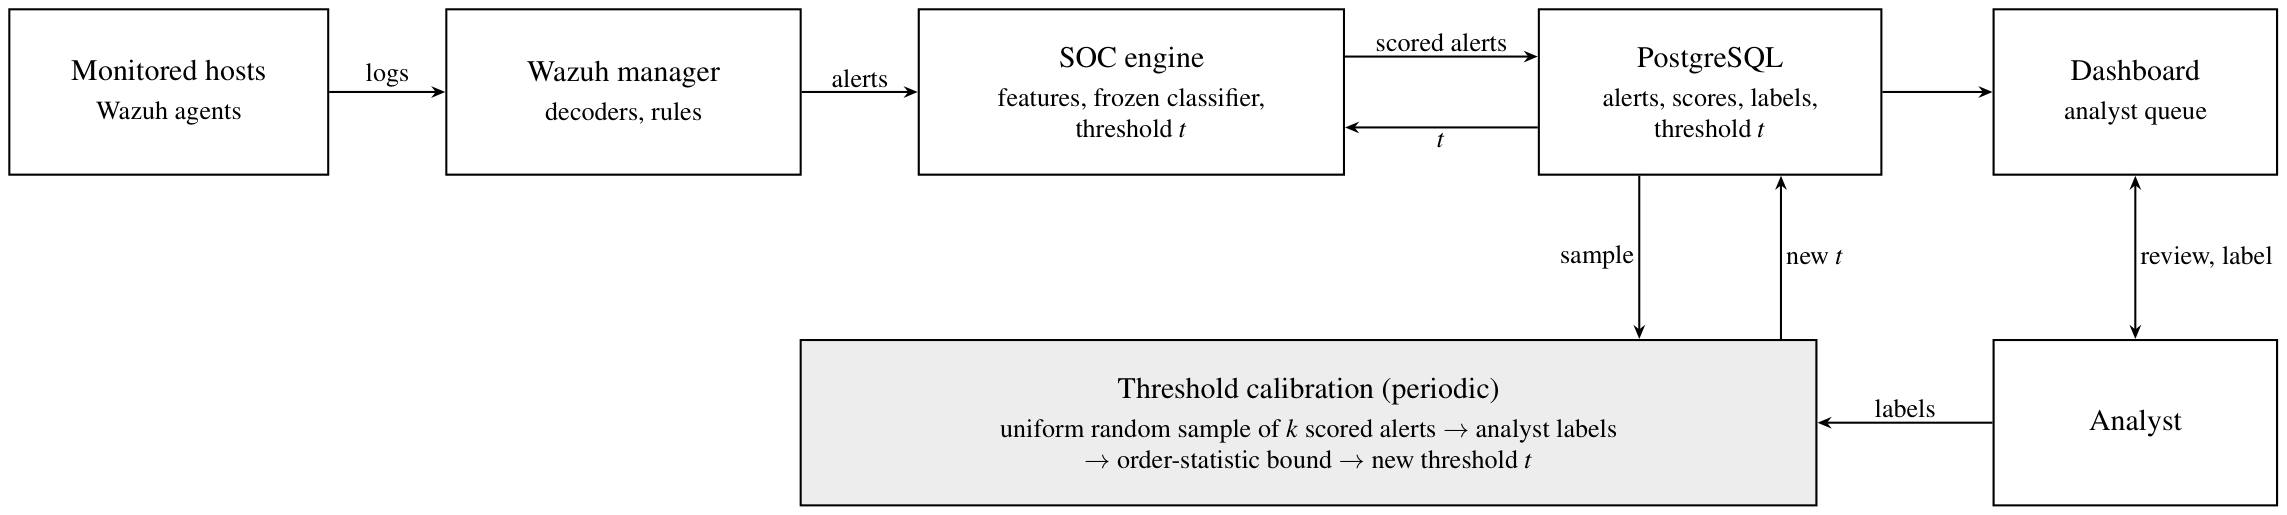
\includegraphics[width=0.92\textwidth]{fig_sys.png}
\caption{System architecture. Wazuh alerts are scored by a frozen classifier and gated by the
threshold $t$; PostgreSQL stores alerts, scores, labels and the threshold. Periodically, a
uniform random sample of scored alerts is labelled by an analyst through the dashboard and the
order-statistic bound writes a new $t$.}
\label{fig:sys}
\end{figure*}

\section{Related Work}

Pietraszek and Tanner~\cite{pietraszek2007} studied learning-based alert post-processing, and
Feng et al.~\cite{feng2017}, Ban et al.~\cite{ban2023}, Kapera and Niemiec~\cite{kapera2025} and
Uetz et al.~\cite{uetz2026} study ML-based triage, volume reduction and risk-based alerting on
proprietary, production or multi-dataset alert data (Table~\ref{tab:related}). Nonparametric tolerance limits date to
Wilks~\cite{wilks1941}; the Neyman--Pearson umbrella algorithm~\cite{tong2018}, risk-controlling
prediction sets~\cite{bates2021} apply such distribution-free ideas to classifiers, but not to alert triage. To our knowledge, none of the
triage studies projects results to realistic attack prevalence, measures how fixed thresholds behave across environments, or
measures how often a few-label rule meets its recall target and at what cost.

\begin{table*}[t]
\centering\footnotesize\setlength{\tabcolsep}{4pt}\renewcommand{\arraystretch}{1.15}
\caption{What each related study evaluates, compared with this paper (from the cited papers'
abstracts and reported results).}
\label{tab:related}
\begin{tabular}{@{}>{\raggedright\arraybackslash}p{4.3cm}>{\raggedright\arraybackslash}p{3.6cm}>{\raggedright\arraybackslash}p{5.0cm}>{\raggedright\arraybackslash}p{4.4cm}@{}}
\toprule
Work & Data & Main evidence reported & Shift or guarantee \\
\midrule
Feng et al.~\cite{feng2017} & one production SOC & ML workflow from labels to risk scores & not addressed \\
Ban et al.~\cite{ban2023} & one real-world network & cost-sensitive learning and event segmentation for IDS alerts & not addressed \\
Kapera, Niemiec~\cite{kapera2025} & one production deployment & 26\% fewer false and repeated alerts & dynamic risk thresholds; no cross-environment test \\
Uetz et al.~\cite{uetz2026} & eight alert datasets & mean AUROC 0.92 (combined hypotheses) vs.\ 0.72 (severity only) & ranking quality only \\
Tong et al.~\cite{tong2018}; Bates et al.~\cite{bates2021} & general classifiers, not alerts & high-probability error control (theory) & guarantees, but not for alert triage \\
\midrule
\textbf{This paper} & own Wazuh deployment (969 alerts) and AIT-ADS (8 scenarios, 391,488 alerts) & prevalence-projected F1; threshold transfer; coverage and label cost of a recall-guaranteed threshold & transfer measured; classical guarantee tested under its assumptions \\
\bottomrule
\end{tabular}
\end{table*}

\section{Data and Setup}

\textbf{Our deployment and data.} Wazuh 4.9.2 on a Google Cloud VM monitors a second VM running
a deliberately vulnerable web app (SQL and OS-command injection, XSS, template injection). Rounds 1--3 used hand-crafted attacks (manual SSH
guessing, curl-based web attacks); round 4 used real tools (hydra, gobuster,
nikto, sqlmap), which trigger Wazuh correlation rules the manual rounds never
did. The dataset has 969 labelled alerts in 26 categories, with labels assigned by us from rules
and known attack scripts (no independent annotator). We train on rounds 1--3 (273 alerts, 6 source
IPs) and test on round 4 (696 alerts, one unseen IP, 82.3\% attacks); the split is time-, IP- and
methodology-disjoint.
\textbf{Features and models.} Each alert is described by its Wazuh severity level
(rule\_level), the hour it occurred, its rule group and decoder, and the words in its log
line (TF-IDF, up to 300 terms, single words and word pairs). IP addresses, ports and timestamps
in the log text are first replaced by placeholders so that models cannot use them as shortcuts.
We compare seven methods: Random Forest (RF; 300 trees, depth 12), logistic regression (LogReg),
a small neural network (MLP; layers of 64 and 32 units), XGBoost (300 trees, depth 6), a simple
cut-off on rule\_level (chosen with Youden's J on the training data), an ensemble that combines the
RF with a recent-alert count and the severity level, and a large language model (LLM) prompted
with and without examples and never shown the true labels. RF, MLP and XGBoost depend on a random seed, so we repeat them (20 runs for RF, 10 for the others) and report mean $\pm$ standard deviation; with only 273 training alerts
their results vary widely. Fig.~\ref{fig:sys} shows the pipeline studied throughout
and Fig.~\ref{fig:rule} how its threshold is calibrated.


\textbf{Public data.} The AIT Alert Data Set~\cite{ait2023,landauer2024} has real Wazuh alerts
from eight simulated enterprise scenarios (2,600,263 alerts). We label an alert an attack if and
only if its timestamp lies in an attack-phase window published with the data set (noisy, window-level labels); no alert-type override is applied, so any alert inside a window,
including scanner ``400 error'' alerts, is an attack here.
We use leave-one-scenario-out evaluation: train on seven scenarios, test on the eighth.

\textbf{Reproducibility.} The source code, the 969-alert labelled dataset, the live-calibration labels
and corrections, and every experiment script with its saved output are maintained on GitHub
(\url{https://github.com/vizarrd/soc-alert-triage-calibration}) and archived on Zenodo (doi:10.5281/zenodo.[number]). A
reproduction guide maps each table and figure to its script, with fixed random seeds and exact package
versions (Python 3.11, scikit-learn 1.9.1). The public AIT data set is not redistributed; it is obtained
from its Zenodo record~\cite{ait2023} and processed by the provided sampling scripts. The LLM runs used
blind sessions of a hosted model and may differ on rerun; raw verdicts are included.

\section{Evaluation Pitfalls on Our Data}

Table~\ref{tab:main} shows round 4 with every method at its default threshold. Because 82.3\%
of the round-4 alerts are attacks, simply calling every alert an attack already gives F1 0.903.
The severity threshold (rule\_level), the LLM and LogReg score about the same
(0.905--0.909), but only because they also flag almost everything: they clear just 2--7\% of the
harmless alerts. Real streams contain far fewer attacks~\cite{axelsson2000}, so we re-estimate each method's results
for a lower attack share $\pi$ from how often it catches attacks (TPR) and raises
false alarms (FPR), assuming both stay the same as the attack share changes, using $P(\pi)=\pi\,\mathrm{TPR}/(\pi\,\mathrm{TPR}+(1-\pi)\,\mathrm{FPR})$
for precision. At $\pi=5\%$ these methods reach only F1 0.10, and an analyst must check about 19
alerts to find one real attack, almost the same as the 20 needed when everything is flagged
(XGBoost is worse: 33). A high F1 therefore hides the problem only when attacks are common.

\begin{table*}[t]
\centering
\caption{Round 4 (train rounds 1--3), default threshold. ``Cleared'' = benign alerts
identified as benign. F1@5\% and review burden (alerts reviewed per real attack) are projected
to 5\% attack prevalence, assuming TPR and FPR stay unchanged. MLP review burden is undefined (some seeds flag nothing).}
\label{tab:main}
\begin{tabular}{@{}lccccccc@{}}
\toprule
Method & F1 & Recall & Cleared & AUC & Relief@R95 & F1@5\% & Review \\
\midrule
rule\_level & .905 & 1.00 & .02 & .966 & .024 & .097 & 19.5 \\
LLM (few-shot) & .905 & 1.00 & .02 & .618 & .024 & .097 & 19.5 \\
LogReg & .909 & 1.00 & .07 & .969 & .935 & .101 & 18.8 \\
XGBoost & .625 & .55 & .08 & .565 & .081 & .057 & 33.1 \\
Random Forest & .47$\pm$.12 & .32$\pm$.09 & .94$\pm$.01 & .404$\pm$.005 & .06$\pm$.01 & .265 & 4.7 \\
Ensemble & .67$\pm$.01 & .51$\pm$.01 & .95 & .556 & .07$\pm$.00 & .420 & 2.8 \\
MLP & .65$\pm$.27 & .56$\pm$.31 & .81$\pm$.37 & .88$\pm$.19 & .69$\pm$.42 & .416 & -- \\
\bottomrule
\end{tabular}
\end{table*}

\textbf{Ranking versus operating point.} Besides the default-threshold results, we judge how
well each method separates attacks from noise at any threshold, using the Triage Relief Curve: the
share of noise cleared against the share of attacks still caught. Its summary, Relief@R95, is the
noise cleared while keeping at least 95\% of attacks. This is just a mirrored ROC curve, not a new
method. The RF clears 94\% of noise at threshold 0.5, but its ROC-AUC is 0.404, below chance: it
calls most unfamiliar traffic benign (recall 0.32) instead of telling the classes apart. The
ensemble beats the RF in all 20 seeds (McNemar $p<10^{-39}$ on seed 0), but that is a better
operating point on a weak ranker (AUC 0.556), not better ranking. LogReg ranks well (AUC 0.969; it clears 93.5\% of
noise while keeping 95\% of attacks); the MLP is unstable across seeds. Training on round 4 and testing on rounds
1--3 gives the same picture: LogReg is best (AUC 0.917) and the RF is poor (0.591).

\textbf{Ensemble.} Following Uetz et al.~\cite{uetz2026}, we combined three signals with a logistic regression
trained on rounds 1--3: the RF probability, the number of alerts from the same source IP in the
previous 10 minutes, and rule\_level. Our first attempt failed (F1 0.15, single run) because this count averages 28 in the training rounds but 342
in the test round, a $12\times$ shift; applying $\log(1+x)$ fixed it (F1 $0.67\pm0.01$, vs.\ $0.47\pm0.12$ for the RF).

\textbf{LLM.} We classified all 696 round-4 alerts with an LLM, given the same fields as our
classifier (rule level and description, decoder, raw log) and blind to ground truth, in seven
independent sessions. A few-shot prompt (told most alerts are benign, eight examples, a probability
output) leaves its decisions unchanged (TPR 1.00, FPR 0.976, AUC 0.618).

\textbf{Label convention.} Of the 123 round-4 benign alerts, 107 are one alert type (``Web server
400 error code'', scanner noise) that we labelled benign by convention. The RF clears all 107 but only 58\% of the other 16; the LLM and rule-level threshold clear none. If scanner
noise is labelled \emph{attack} instead, the rule-level threshold and LLM become essentially
correct (recall 1.00), the RF's recall drops (0.32 to 0.27) and AUCs change (rule level 0.97 to
0.85, LogReg 0.97 to 0.72), so round-4 method comparisons are convention-dependent.

\section{Cross-Environment Behaviour on Public Data}

\label{sec:ait}

Table~\ref{tab:ait} shows results on the public data. Each of the eight scenarios is held out in
turn and the models are trained on the other seven, using a random sample of 4,000 alerts per
scenario (6.8--88.6\% attacks). One caveat applies throughout: an alert counts as an attack if it falls inside a published attack time window, not
because anyone checked that the alert itself is malicious.

\begin{table}[!h]
\centering
\caption{AIT-ADS, mean over 8 held-out scenarios. ``Transfer'': threshold from out-of-fold
training scores for 95\% recall. ``+20'': re-thresholded with 20 labelled target alerts.}
\label{tab:ait}
\resizebox{\ifdim\width>\columnwidth\columnwidth\else\width\fi}{!}{\begin{tabular}{@{}lccccc@{}}
\toprule
Model & AUC & Relief@R95 & Transfer recall / cleared & +20 recall / cleared \\
\midrule
rule\_level & .692 & .339 & .94 / .69 & .94 / .54 \\
LogReg & .960 & .695 & .84 / 1.00 & .86 / .86 \\
Random Forest & .964 & .735 & .81 / 1.00 & .93 / .84 \\
MLP & .957 & .660 & .92 / 1.00 & .87 / .83 \\
\bottomrule
\end{tabular}}
\end{table}

\textbf{LLM versus trained models.} Methods that read the log content beat the rule\_level
threshold clearly (AUC 0.96 versus 0.69). The LLM was run on a smaller sample of 150 alerts per
scenario (1,200 alerts in total), taken from the 4,000-per-scenario sample behind
Table~\ref{tab:ait}, so its scores cannot be compared with that table or with results on all
32,000 alerts. For a fair comparison we therefore scored the trained models (each trained on the
other seven scenarios) on exactly the same 1,200 alerts. The mean AUC per scenario is 0.959 for
the LLM, against 0.950 for LogReg, 0.954 for RF and 0.947 for MLP; the rule-level threshold is far
behind. To check whether these small gaps are real, we resampled the alerts and the scenarios many
times (bootstrap). The 95\% intervals for the LLM's advantage are narrow and mostly include zero
against the trained models (for example $-0.009$ to $+0.027$ against LogReg), but are large
against the rule-level threshold ($+0.22$ to $+0.31$). The LLM beats LogReg, RF and MLP in only
4, 2 and 3 of the 8 scenarios, and beats the rule-level threshold in all 8. We therefore do not
claim a winner: the LLM is on par with the trained models and clearly better than the rule-level
threshold. It also does not simply flag everything; on our own data it did so because of the
labelling convention described above. Removing feature groups from LogReg shows why the datasets differ: on the public data no single
group matters much (AUC stays at 0.958--0.962; the severity level alone gives only 0.692), while on
our data the severity level alone gives 0.966, dropping it gives 0.397 and the log text alone
0.334 (below chance). The public data is also easier: 90\% of its attack-labelled alerts are the
``Web server 400 error'' alert, which \emph{our own} dataset labels benign, so the two datasets
use opposite conventions for scanner noise.

\textbf{Thresholds do not transfer.} On our data, a 95\%-recall threshold chosen on rounds
1--3 makes LogReg and rule\_level flag everything on round 4 (noise cleared 6.5\%
and 2.4\%) because attack prevalence moves from 20\% to 82\%~\cite{saerens2002}. On AIT, transferred thresholds
clear nearly all noise but miss the recall target (0.81--0.92 on average; RF 0.00 on shaw). Re-thresholding with 20 random labels
helps the worst case (RF on shaw: 0.00 to 0.82) only partly.



\begin{figure}[t]
\centering
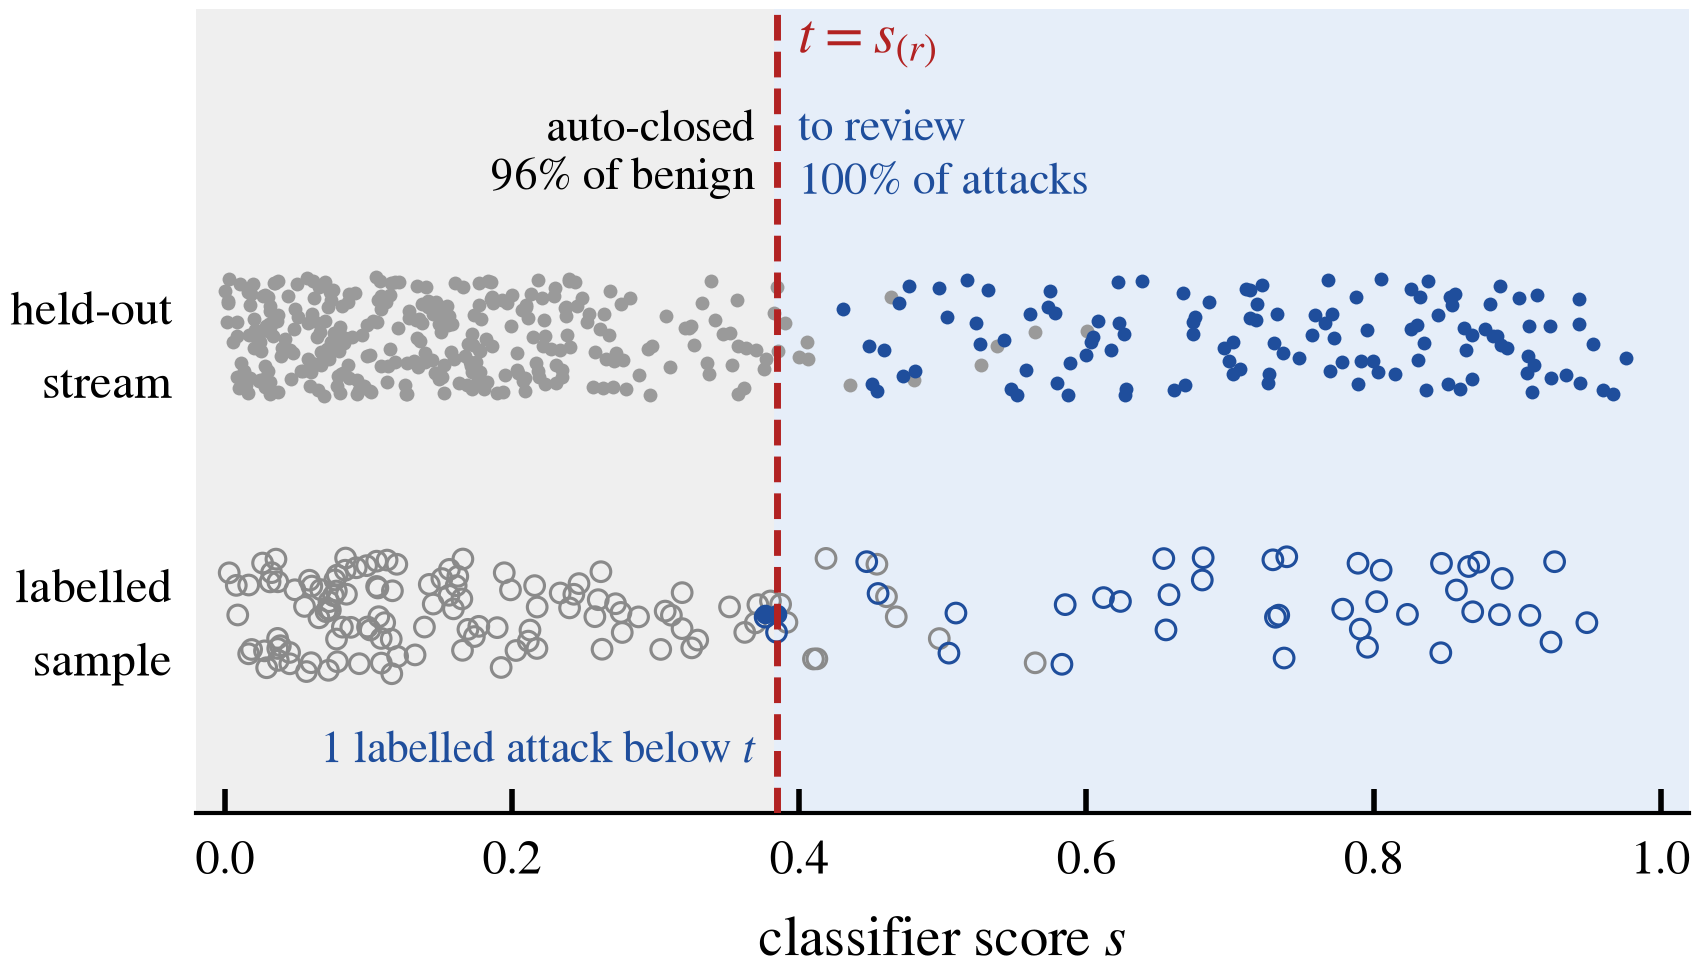
\includegraphics[width=\columnwidth]{fig_rule_a.png}
\caption{How the threshold is obtained (illustrative seeded simulation, not experimental data): $k=160$ uniformly drawn alerts are labelled ($n=39$ attacks; filled dots mark the $r$ lowest). The $r$-th lowest labelled attack score is the threshold $t$; held-out alerts below it are auto-closed.}
\label{fig:rule}
\end{figure}

\section{A Recall-Guaranteed Threshold}
\label{sec:guarantee}

\textbf{Rule.} Draw $k$ alerts at random and have an analyst label them; $n$ of them turn out
to be attacks, with model scores $s_{(1)}\le\dots\le s_{(n)}$ (sorted). Let
$\rho$ be the share of attacks we want to catch (target recall) and $\delta$ the chance we allow
of missing that target. Choose the largest rank $r\le n$ for which
$\Pr[\mathrm{Beta}(r,n-r+1)\le 1-\rho]\ge 1-\delta$, set the threshold to $t=s_{(r)}$ (the
$r$-th lowest attack score), and flag every alert that scores at least $t$. If no such $r$ exists,
there are too few labelled attacks, so we flag everything ($t=-\infty$, the \emph{fallback}).
Certification needs at least $\lceil\ln\delta/\ln\rho\rceil$ labelled attacks (22 for
$\rho=0.9$, $\delta=0.1$), which is about $22/p$ labelled alerts when a share $p$ of the alerts
are attacks. This is a classical one-sided tolerance bound~\cite{wilks1941}, as in the Neyman--Pearson umbrella
algorithm~\cite{tong2018} (there it bounds type-I error, here the miss rate); our contribution is applying and
evaluating it for alert triage. \emph{Intuition} (Figs.~\ref{fig:rule} and~\ref{fig:rule2}): the
lowest scores among the labelled attacks show where the attack scores start. The more attacks are
labelled, the higher a rank $r$ we can pick while still being 90\% sure that at most 10\% of all
attacks score below $t$.


\textbf{Guarantee.} \emph{Assume (A1) the $k$ labelled alerts are a uniform random sample of the
alert stream, (A2) the analyst's labels are correct, and (A3) the model and its scores do not
change afterwards. Then, for the number $n$ of labelled attacks we have, the recall at threshold
$t$ is at least $\rho$ with probability at least $1-\delta$.} The reason is standard. If the $n$
labelled attack scores are independent draws from all attack scores, the share of attacks scoring
below $s_{(r)}$ follows a Beta$(r,n-r+1)$ distribution, and recall at $t$ is at least one minus
that share. Tied scores can only raise recall, never lower it. In our experiments the labelled alerts are instead drawn without
replacement from a finite stream, where the exact probabilities follow a hypergeometric law. We
still use the Beta rule, because in practice the number of attacks in the stream is unknown. To
check it, we computed the exact success probability of the rule under this sampling for 8,775
settings ($n$ from its minimum up to 1,000; $\rho\in\{0.80,0.90,0.95\}$; $\delta=0.10$; streams
with 3,426, 10,000 or 44,524 attacks), assuming no tied scores; it never fell below 0.9007. This
is a numerical check on that grid, not a general proof, and the coverage experiments below remain
the direct empirical test. The guarantee concerns the attacks in the stream under (A1)--(A3), not
every future deployment: if the data drift, the rule must be re-run (we did not test this). It
covers recall only; noise cleared is an empirical outcome.

\begin{figure}[b]
\centering
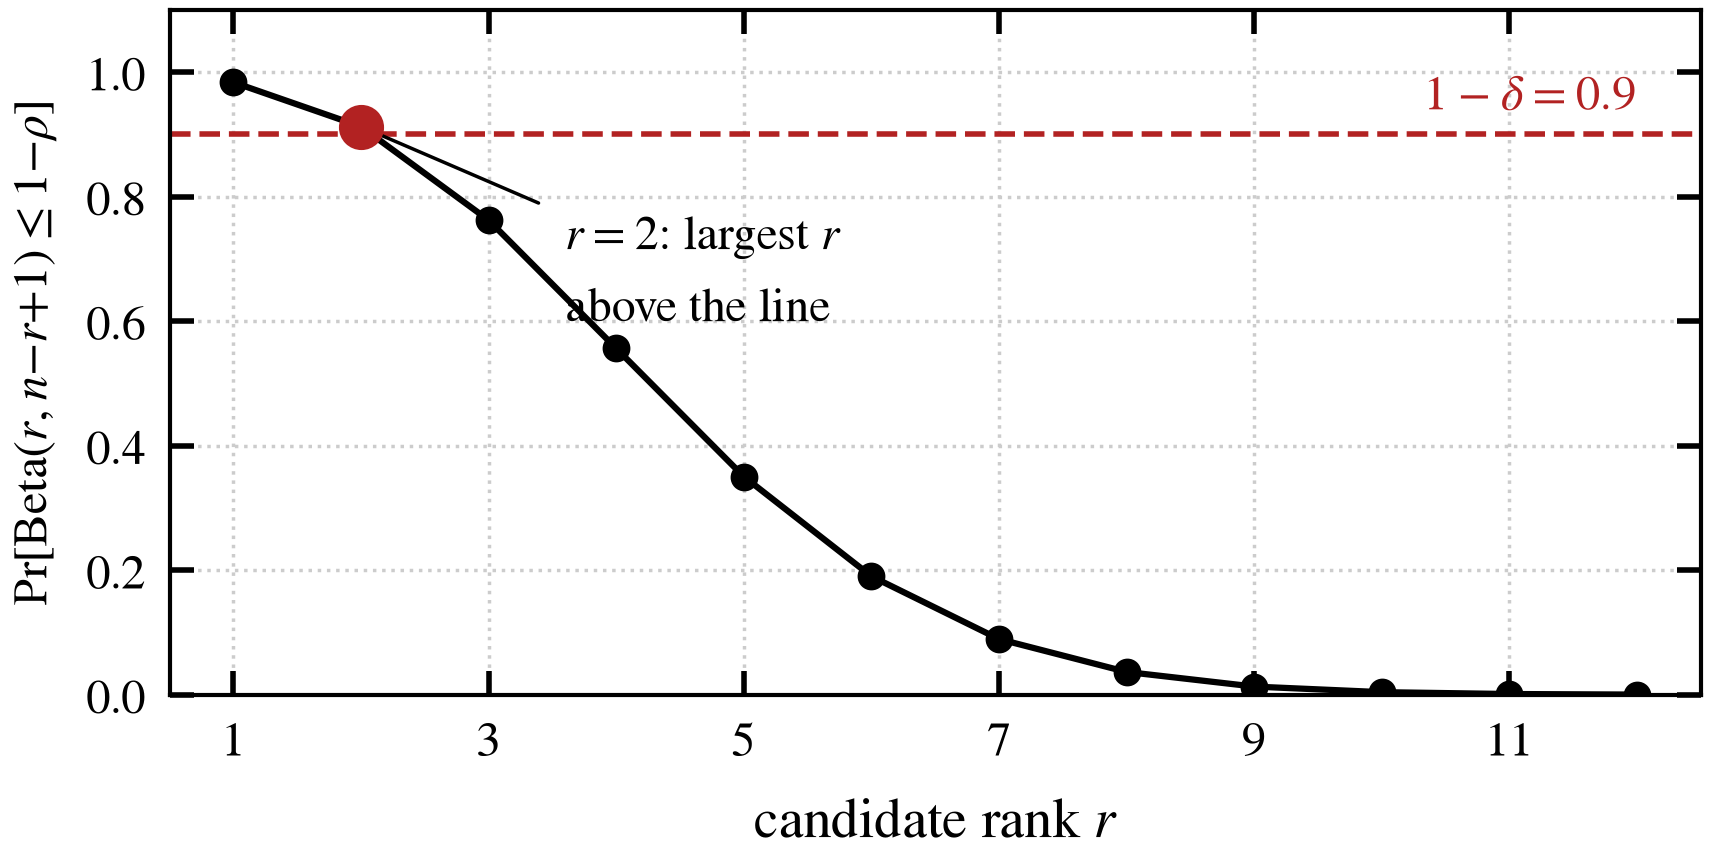
\includegraphics[width=\columnwidth]{fig_rule_b.png}
\caption{Choosing $r$: the largest rank for which $\Pr[\mathrm{Beta}(r,n{-}r{+}1)\le 1{-}\rho]\ge 1-\delta$ ($n=39$, $\rho=0.9$, $\delta=0.1$).}
\label{fig:rule2}
\end{figure}

\begin{table*}[!t]
\centering\footnotesize\setlength{\tabcolsep}{4.5pt}
\caption{Coverage and cost of the guaranteed threshold on the large AIT-ADS streams (LogReg;
$\rho=0.90$, $\delta=0.10$; 1{,}000 trials per scenario and $k$). $\hat c$: share of certified
trials ($N_{\mathrm{cert}}$) with true recall $\ge\rho$, with 95\% Wilson interval;
$\hat c_{\mathrm{all}}$ also counts uncertified trials (flag all) as successes; Uncert.: share of
trials without a certificate. Guarantee-check columns use the $S$ scenarios with $\ge100$ certified
trials at that $k$; cost columns average all 8 scenarios and must not be combined with them.
$^{\dagger}$Trivial. Bold: interval above 0.90.}
\label{tab:large}
\begin{tabular}{@{}llcccccccc@{}}
\toprule
 & & \multicolumn{5}{c}{Guarantee check (same $S$ scenarios)} & \multicolumn{2}{c}{Cost (all 8 scenarios)} \\
\cmidrule(lr){3-7}\cmidrule(lr){8-9}
Rule & $k$ & $S$ & $N_{\mathrm{cert}}$ & $\hat c$ [95\% CI] & $\hat c_{\mathrm{all}}$ & Uncert. & Benign cleared & Uncert. \\
\midrule
Flag everything & -- & -- & -- & $1.000^{\dagger}$ & -- & -- & 0.00 & -- \\
Naive threshold & 200 & 8 & 8{,}000 & 0.525 [0.514, 0.536] & 0.525 & 0.00 & 0.87 & 0.00 \\
Naive threshold & 1000 & 8 & 8{,}000 & 0.619 [0.608, 0.630] & 0.619 & 0.00 & 0.87 & 0.00 \\
\midrule
Guaranteed & 50 & 4 & 4{,}000 & \textbf{0.961} [0.955, 0.967] & 0.961 & 0.00 & 0.46 & 0.50 \\
Guaranteed & 100 & 5 & 4{,}425 & \textbf{0.940} [0.933, 0.947] & 0.947 & 0.12 & 0.52 & 0.45 \\
Guaranteed & 200 & 6 & 5{,}182 & \textbf{0.944} [0.937, 0.950] & 0.952 & 0.14 & 0.56 & 0.34 \\
Guaranteed & 500 & 8 & 7{,}989 & \textbf{0.952} [0.947, 0.956] & 0.952 & 0.00 & 0.66 & 0.00 \\
Guaranteed & 1000 & 8 & 8{,}000 & \textbf{0.955} [0.950, 0.959] & 0.955 & 0.00 & 0.72 & 0.00 \\
\bottomrule
\end{tabular}
\end{table*}

\textbf{Experiments.} We keep three things apart: the mathematical guarantee (which holds under
A1--A3), how often it actually held in simulated labelling runs (this section), and whether it
holds in real deployments, which we have not established (Section~\ref{sec:live}). A \emph{trial}
draws $k$ random alerts, labels them, sets the threshold with the rule, and checks whether the true
recall on the whole stream is at least $\rho$. \emph{Coverage} is the share of trials in which
this succeeds. A trial with fewer than 22 labelled attacks cannot be certified and falls back to
flagging everything, which trivially gives recall 1. We therefore check the guarantee on certified
trials only (Table~\ref{tab:large}) and also report the numbers with all trials included. In a first study (LogReg, 100 trials), a naive rule that keeps the fraction $\rho$ of the labelled attacks reached recall 0.90 in only
0.58--0.83 of trials with 20--100 labels, and choosing the alerts to label more cleverly did not help (stratified 0.60--0.84, uncertainty 0.50--0.75).



\textbf{Large-scale check and provenance.} The public data holds 2,600,263 alerts; from each
scenario we drew up to 50,000 uniformly without replacement (391,488 distinct alerts;
russellmitchell in full), and used 1,000 random labelling trials for each of 240 settings (8
scenarios, 2 models, 5 values of $k$, 3 values of $\rho$). Recall and noise cleared are true
values on the whole held-out stream. The alerts are time-correlated; this does not affect the guarantee,
whose target is the uniformly sampled finite stream, but the evidence rests on eight
scenarios.



\textbf{Results.} Fig.~\ref{fig:guar} shows the picture per scenario. Counting uncertified trials
as successes changes the coverage by at most 0.008 (Table~\ref{tab:large}; largest raw difference
0.0076, at $k=200$), so the certified numbers are not an artifact of leaving trials out. We look
at the 184 of 240 settings that have at least 100 certified trials. The target is 0.90, and the
average certified coverage is well above it: 0.965 for the 90\% recall target (62 settings), 0.983
for the 80\% target (72 settings) and 0.967 for the 95\% target (50 settings; lowest 0.906). Two
settings fell slightly below 0.90: 0.899 at the 90\% target (RF on shaw, $k=200$; 95\% Wilson
interval [0.84, 0.94], 148 certified trials) and 0.862 at the 80\% target (LogReg on santos,
$k=100$; [0.79, 0.91], 116 trials). Neither interval lies entirely below 0.90; we keep both results. Because they looked low, we reran them with 10,000 trials, a fresh training
sample, and recall measured on alerts that were not in the labelled sample. The reruns gave 0.936
[0.92, 0.95] (1,565 certified trials) and 0.930 [0.92, 0.94] (1,363). We reran these two settings
precisely because they looked low, which favours higher rerun values, so the reruns support, but
do not prove, that the dips were random sampling noise. These are simulation estimates, not a proof.

\textbf{Is the guarantee worth its cost?} Compare three ways of achieving the same goal (recall
0.90). Flagging everything always meets it but clears nothing. The naive rule clears 0.87 of the
benign alerts (analysts still review 13\%), but it meets the target in only about half of the
trials (coverage 0.32--0.80), as expected for a rule that aims exactly at the target. The
guaranteed rule achieves a certified coverage above 0.9, but clears only 0.46--0.72 of the benign
alerts (analysts review 28--54\%). The guarantee is therefore worth paying for when missing an
attack is costly and enough labels are available. It needs many labels when attacks are
rare: at least $22/p$ labelled alerts at attack share $p$ (2,200 at 1\%, 440 at 5\%, 220 at 10\%); in our
7--9\% scenarios about 500 were needed. The naive rule is cheaper if occasional misses are acceptable.

\section{Live Deployment}
\label{sec:live}

\begin{figure*}[!t]
\centering
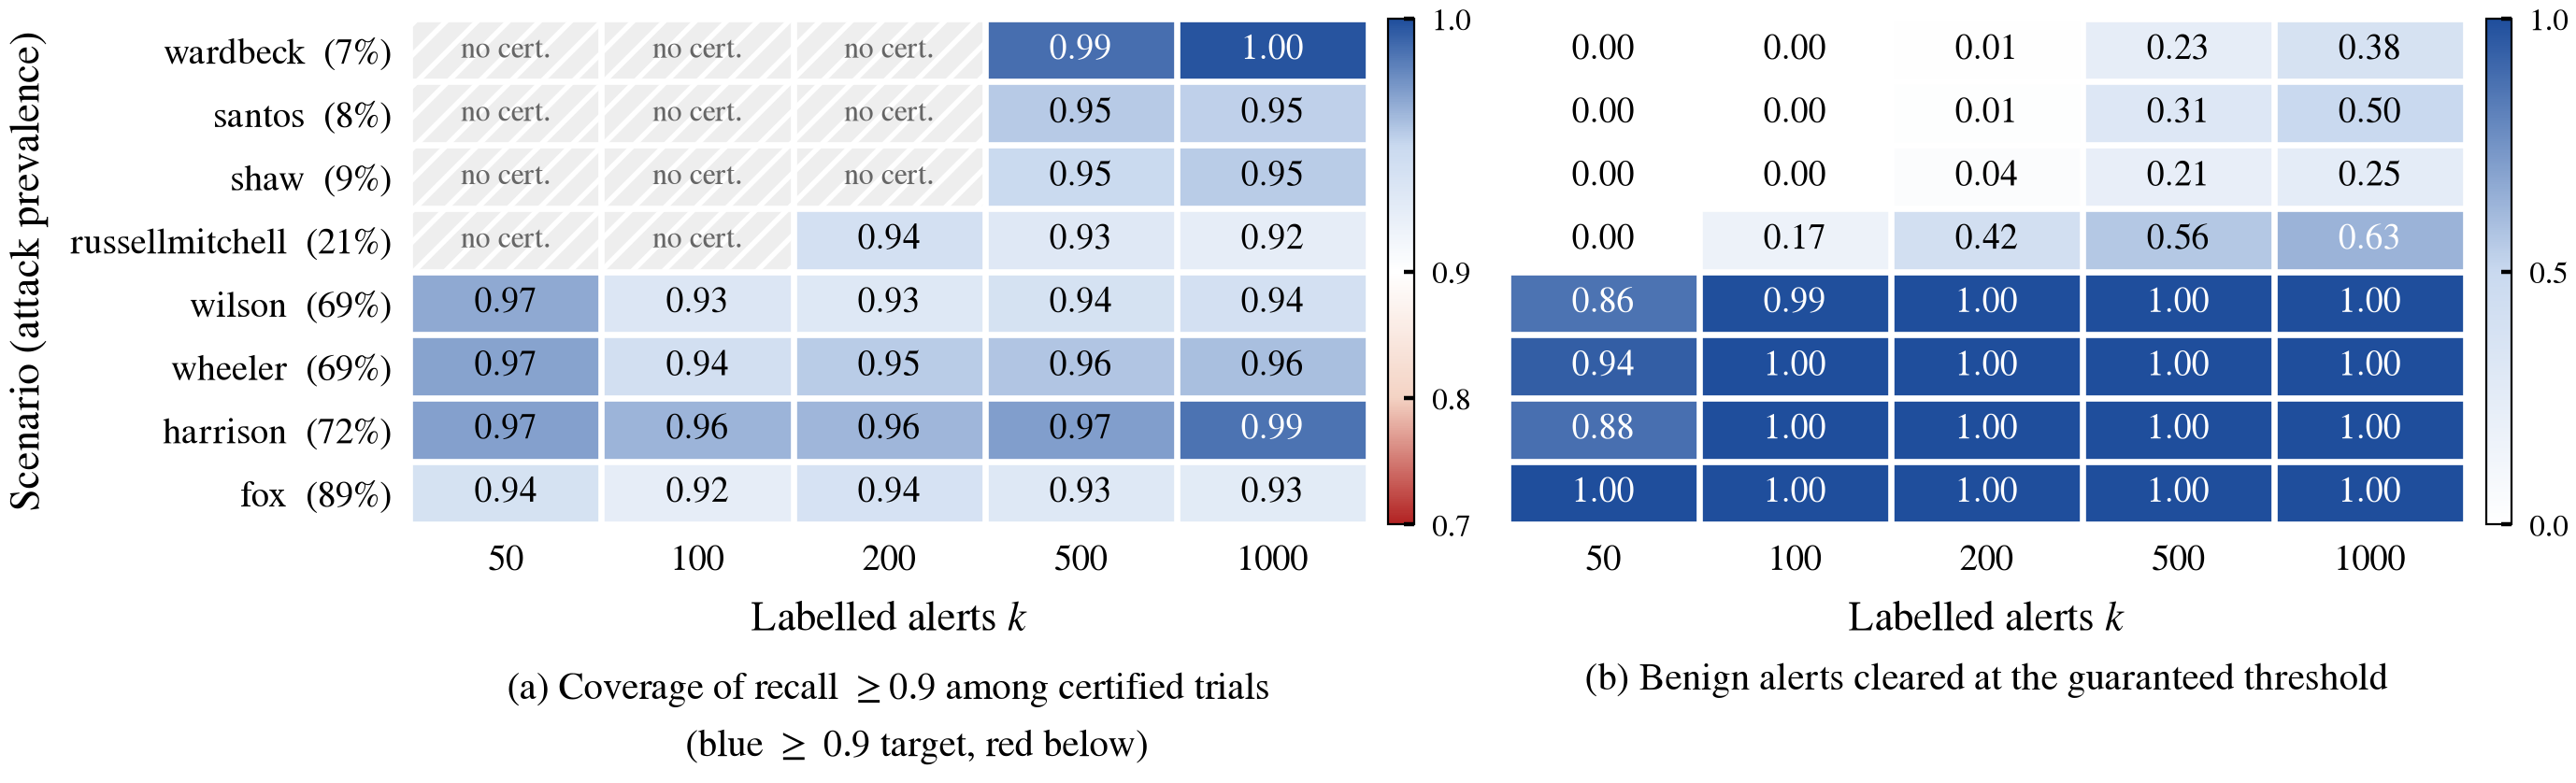
\includegraphics[width=0.88\textwidth]{fig_heat.png}
\caption{The guarantee study per scenario (LogReg, $\rho=0.90$, 1{,}000 labelling trials per cell;
scenarios sorted by attack prevalence). (a) Coverage among certified trials: all certified cells shown
are $\ge 0.90$ (blue); hatched: too few labelled attacks ($n<22$) to certify. (b) Benign alerts
cleared at the guaranteed threshold: near zero for rare-attack scenarios, about 1 for attack-heavy ones.}
\label{fig:guar}
\end{figure*}

We deployed the system on Google Cloud (Wazuh, the classifier, PostgreSQL and a web dashboard).
One analyst labelled randomly selected alerts in the dashboard over two rounds, covering attacks we
launched and real internet SSH bots. Until 22 attacks have been labelled, the system reports itself
as \emph{uncalibrated} (default threshold 0.5, no guarantee); thereafter it applies the
recall-guaranteed threshold of Section~\ref{sec:guarantee}.

\textbf{Round 1.} With a LogReg model trained on our 969 alerts, 43 labels (36 attacks, after we
corrected three routine package-update alerts that had been marked as attacks) certified a
threshold of 0.0004, so nearly every alert was flagged. The lowest-scoring labelled attack was a
real SSH-bot event (``PAM: User login failed'') that the model scored 0.0004, because our training
data labelled such events benign. The guarantee held, but exposed a blind spot in the model. Retraining with the 43 live labels (weighted 5) raised the lowest held-out attack score from
0.0004 to 0.022 in cross-validation, but held-out ROC-AUC fell (0.795 to 0.767): the blind spot was removed without improving ranking.

\textbf{Round 2.} With the retrained model and fresh labels, the analyst marked all 28 sampled
alerts as attacks, including seven routine ``PAM login session opened/closed'' events that we
classify as benign. We corrected six of these (originals kept) and left
the seventh. The system certified at 22 attacks with a threshold of 0.0665, set by that remaining
routine alert, and flagged 211 of 229 scored alerts (92\%), against 156 (68\%) at the default
threshold of 0.5. Because the weakest labelled attack sets the threshold, one routine alert labelled as an attack
removes almost all noise reduction, and the guarantee needs correct labels (A2). Nine of 71 live labels (13\%) required correction.
The deployment shows that the loop runs end to end with only a few dozen labels, and that the
lowest-scoring labelled attacks act as a diagnostic: they point directly to what the model
misses (Round 1) and to labels worth re-checking (Round 2).

\section{Discussion and Limitations}

Our comparison does not show that LLMs are better or worse than trained classifiers: their ranking differed between datasets. Likewise, the coverage results come from
simulation and should not be read as evidence of production reliability, nor of recall under
distribution shift, label noise or changed attacker behaviour.

\textbf{Limitations.} Both datasets are Wazuh-based and use rule-based or window-level labels.
Our own dataset has seven source IPs, a narrow benign class (107 of 123 alerts are of one type) and
labels from a single party, while the public dataset is comparatively easy: rule type nearly
determines the label. The results should therefore not be assumed to generalize to
other SOC environments. The labels were not independently validated. The guarantee
assumes random samples, correct labels and no drift; in deployment we tested it with a single
analyst only. These limits define the scope of our claims.

\section{Conclusion}

We asked whether the usual ways of judging alert-triage tools still hold when a tool moves to a
new environment. On our own Wazuh deployment and on the public AIT data, they often do not. First,
a high F1 can simply mean that almost every alert is flagged; at realistic attack rates such a
system gives analysts nearly as much work as flagging everything. Second, results do not travel:
the ranking of an LLM, a rule-level threshold and trained classifiers differed between the two
datasets, and a threshold chosen in one environment missed attacks in another. Third, a classical
order-statistic rule can set the threshold from a small random sample of analyst-labelled alerts.
Once enough attacks are labelled (22 for a 90\% target), its recall guarantee held in 96.5\% of
simulated labelling trials on average over streams of 391,488 alerts, at the price of clearing
fewer harmless alerts and of needing hundreds of labels when attacks are rare. The guarantee
relies on random samples, correct labels and a stable model; in our live deployment 13\% of labels
needed correction, so we show the workflow, not a validated live guarantee. In practice we
therefore suggest reporting results at realistic attack rates, re-calibrating the threshold with
a few random labels whenever the environment changes, and checking labels before trusting the
guarantee. Testing the approach on larger, independently labelled production alert streams is the
main next step.

\begin{thebibliography}{00}
\bibitem{alahmadi2022} B.~A. Alahmadi, L.~Axon, and I.~Martinovic, ``99\% false positives: A
qualitative study of SOC analysts' perspectives on security alarms,'' in \emph{31st USENIX
Security Symp.}, 2022, pp.~2783--2800.
\bibitem{feng2017} C.~Feng, S.~Wu, and N.~Liu, ``A user-centric machine learning framework
for cyber security operations center,'' in \emph{Proc. IEEE ISI}, 2017, pp.~173--175,
doi:10.1109/ISI.2017.8004902.
\bibitem{ban2023} T.~Ban, T.~Takahashi, S.~Ndichu, and D.~Inoue, ``Breaking alert fatigue:
AI-assisted SIEM framework for effective incident response,'' \emph{Appl. Sci.}, vol.~13,
no.~11, p.~6610, 2023, doi:10.3390/app13116610.
\bibitem{kapera2025} A.~Kapera and M.~Niemiec, ``Dynamic risk thresholds for SIEM alerting
based on machine learning,'' \emph{IEEE Access}, vol.~13, pp.~121034--121047, 2025,
doi:10.1109/ACCESS.2025.3588441.
\bibitem{uetz2026} R.~Uetz, P.~B{\"o}nninghausen, L.~Hackl{\"a}nder-Jansen, and M.~Henze,
``Can risk-based alerting mitigate cybersecurity alert fatigue?'' arXiv:2609.02465, 2026.
\bibitem{xu2024llmsec} H.~Xu \emph{et al.}, ``Large language models for cyber security: A
systematic literature review,'' arXiv:2405.04760, 2024.
\bibitem{arp2022} D.~Arp, E.~Quiring, F.~Pendlebury, A.~Warnecke, F.~Pierazzi, C.~Wressnegger,
L.~Cavallaro, and K.~Rieck, ``Dos and don'ts of machine learning in computer security,'' in
\emph{Proc.\ 31st USENIX Security Symp.}, Boston, MA, USA, Aug.\ 2022.
\bibitem{ait2023} M.~Landauer, F.~Skopik, and M.~Wurzenberger, ``AIT Alert Data Set,''
Zenodo, 2023, doi:10.5281/zenodo.8263181.
\bibitem{landauer2024} M.~Landauer, F.~Skopik, and M.~Wurzenberger, ``Introducing a new alert
data set for multi-step attack analysis,'' in \emph{Proc. CSET}, 2024,
doi:10.1145/3675741.3675748.
\bibitem{wilks1941} S.~S. Wilks, ``Determination of sample sizes for setting tolerance
limits,'' \emph{Ann. Math. Statist.}, vol.~12, no.~1, pp.~91--96, 1941.
\bibitem{tong2018} X.~Tong, Y.~Feng, and J.~J. Li, ``Neyman--Pearson classification algorithms
and NP receiver operating characteristics,'' \emph{Sci. Adv.}, vol.~4, no.~2, p.~eaao1659, 2018.
\bibitem{pietraszek2007} T.~Pietraszek and A.~Tanner, ``Data mining and machine
learning---towards reducing false positives in intrusion detection,'' \emph{Inf. Secur.
Tech. Rep.}, vol.~10, no.~3, pp.~169--183, 2005, doi:10.1016/j.istr.2005.07.001.
\bibitem{bates2021} S.~Bates, A.~Angelopoulos, L.~Lei, J.~Malik, and M.~I. Jordan,
``Distribution-free, risk-controlling prediction sets,'' arXiv:2101.02703, 2021.
\bibitem{axelsson2000} S.~Axelsson, ``The base-rate fallacy and the difficulty of intrusion
detection,'' \emph{ACM Trans.\ Inf.\ Syst.\ Secur.}, vol.~3, no.~3, pp.~186--205, Aug.\ 2000.
\bibitem{saerens2002} M.~Saerens, P.~Latinne, and C.~Decaestecker, ``Adjusting the outputs of a
classifier to new a priori probabilities: A simple procedure,'' \emph{Neural Comput.}, vol.~14,
no.~1, pp.~21--41, 2002, doi:10.1162/089976602753284446.
\end{thebibliography}

\end{document}
